% multiple1902 <multiple1902@gmail.com>
% intro.tex
% Copyright 2011~2012, multiple1902 (Weisi Dai)
% https://code.google.com/p/xjtuthesis/
%
% It is strongly recommended that you read documentations located at
%   http://code.google.com/p/xjtuthesis/wiki/Landing?tm=6
% in advance of your compilation if you have not read them before.
%
% This work may be distributed and/or modified under the
% conditions of the LaTeX Project Public License, either version 1.3
% of this license or (at your option) any later version.
% The latest version of this license is in
%   http://www.latex-project.org/lppl.txt
% and version 1.3 or later is part of all distributions of LaTeX
% version 2005/12/01 or later.
%
% This work has the LPPL maintenance status `maintained'.
%
% The Current Maintainer of this work is Weisi Dai.
%

\chapter{论文相关理论与技术}
\echapter{Relative Theory and Technology}

    文字检测按照其研究目标和存储介质的不同,可分为数字图像文字检测、视频图像中的文字检测和自然场景图像中的文字检测。其中,由于自然场景中的文字会遭受背景复杂多样性,以及图像质量易被光照、阴影、遮挡等环境因素影响,致使自然场景图像的文字检测相比于其它图像对检测算法的健壮性要求更高。这些年来,学者们在文字检测领域进行了大量的研究和实验工作,提出了许多不同的方法,检测效果也在逐年提升。但是在ICDAR等公开数据集上的测试结果表明,目前的这些自然场景图像中的文字检测结果仍有提高空间,所以仍是文字检测领域内的一个热点方向。场景图像文字检测方法根据流程不同,可分为基于区域的文字检测方法和基于连通部件的文字检测方法两大类。下面整理并分别介绍近年来这两类文字检测的相关方法。

    \section{基于区域的场景文字检测方法}
    \esection{Region-based Method}

    基于区域的文字检测方法,是基于文子有别于背景的视觉特征来区分文字区域与背景区域的。使用较多的视觉特征主要包括纹理、边缘及颜色等。因为每个文字都是用来传递信息的特定符号,其纹理与一般背景并不相同,同时文字相比于背景也有着更强的对比度和显著的颜色,所以包含着文字的那些区域和背景图像区域有着不同的视觉特征,因而可以用来区分文字区域与非文字区域。

    大部分基于区域的方法一般都会利用滑动窗来获取候选的包含文字的局部图像区域,因此在有些方法中也称其为基于滑动窗的文字检测算法。如图\ref{fig.c2_region_based} 所示,这是1 个典型的基于区域的文字检测方法的步骤示例。在该步骤示例中,首先利用滑动窗来得到局部图像区域以作为候选区域,然后提取区域中的颜色、纹理等视觉特征,最后结合分类器以进行文字与非文字区域的分类判别,输出结果是检测出来的文字区域。

    \begin{figure}[!h]
    \centering
    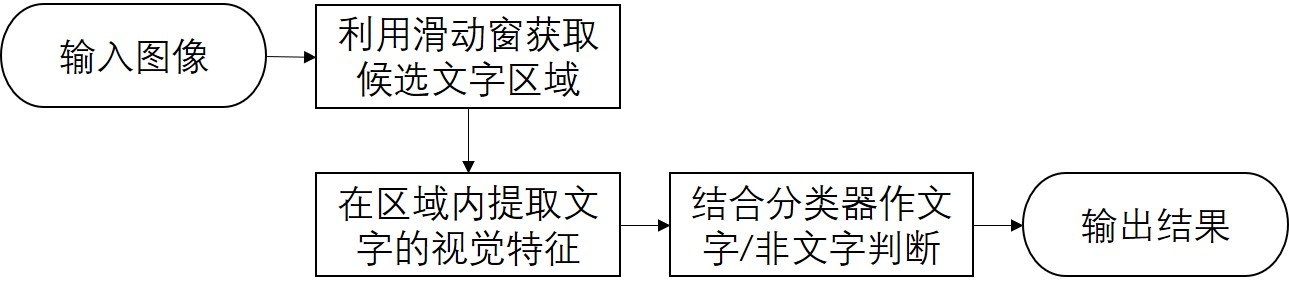
\includegraphics[width=\textwidth]{c2_region_based.jpg}
    \caption{基于区域的文字检测方法的步骤示意图}
    \label{fig.c2_region_based}
    \end{figure}

    Chen等\cite{Chen2004Detecting}利用滑动窗扫描得到文字区域并获取区域中的79 个特征,然后构造4 个级联的Adaboost 分类器来分类和筛选这些候选文字区域,最后用OCR软件识别图像中文字信息。其中4 个级联的分类器是由不同的文字底层特征构造而成的弱分类器,通过利用Adaboost 方法将这些弱分类器组合学习而获得1 个分类文字与背景的强分类器。用于训练弱分类器的三组特征分别是:候选区域内竖直和水平方向灰度的标准差与平均值;区域内的统计梯度信息;区域内边缘组合特征。而本方法中使用的79 个特征,分散在4 层的级联分类器中,分别有1、10、30和50 维文字特征。最后OCR 使用的技术是用Niblack 方法来二值化检测到的文字区域以识别出图像中的文字。

    Pan等\cite{Pan2011A}设计了一种基于滑动窗的文本区域的检测器,用于估算图像金字塔中的文本行存在的置信度和尺度信息,在每个尺度中使用滑动窗扩得到候选文字区域并利用WaldBoost 分了器对各个窗口的文字置信度进行预测。然后该文利用基于连通部件类别中的局部二值化方法对候选文本分量进行分割。为有效的过滤掉非文本的部件,这篇文章提出了一个考虑一元组件的属性和二元上下文的成分关系的条件随机场(CRF)模型。其中,一元特征表征单个部件自身的文字置信度,例如有占空比、紧密度、轮廓梯度以及宽高比等;而二元特征表征相邻候选文字连通部件即上下文的关系,如颜色、形状、尺度和距离等差异。最后基于能量最小化方法将这些文本组件分类到文本行中。

    上述文字检测方法一般使用人工设计的特征,例如颜色、纹理、笔画宽度等,进行文字与非文字分类。虽然这些特征可以区分大多数的文字与非文字,部分与文字相似的背景却难以区分,例如窗户、砖块等。为了能够更好地反映文字的属性,近年来许多方法开始采用深度学习技术,其中最常用的一种结构是卷积神经网络(CNN)。CNN是一种特殊的前馈人工神经网络,其中的神经元之间的连接关系类似于视觉皮层的结构。同时,因为CNN能够利用图像中的局部空间相关性,故CNN特别适合于处理计算机视觉问题,尤其是目标识别领域,例如在手写字符识别、交通标志识别、图像分类等方面都取得了优秀的表现。

    \begin{figure}[!h]
    \centering
    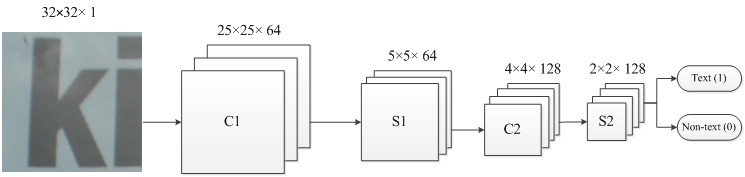
\includegraphics[width=\textwidth]{c2_wangtao_cnn.jpg}
    \caption{Wang等\cite{Wang2012End} 采用的CNN 网络框架}
    \label{fig.c2_wangtao_cnn}
    \end{figure}

    Wang等\cite{Wang2012End}设计的端对端文字检测和识别框架的核心即是卷积神经网络CNN。该方法首先利用滑动窗在图像金字塔上扫描得到候选文字图像块区域,然后将这些图像块区域缩放成$32\times32$ 像素大小的正方形小图块。接着这些图块的灰度图会输入到1 个训练好的,含有2 层卷积的CNN 网络中进行特征的提取,以及对这些图块区域的分类。其中,卷积神经网络CNN的结构如图\ref{fig.c2_wangtao_cnn} 所示:输入图像小块经过第1层的64个卷积模板的卷积操作后,得到64个$25\times25$的响应图,紧接着再执行平均池化获得相应的$5\times5$ 的响应;然后再通过第2卷积层中的128个卷积模板的卷积操作及后续的平均池化操作后,得到$2\times2\times128$ 的全连接层。在通过上CNN 网络的特征提取和分类后,最后再利用非极大抑制NMS 操作来筛选重叠的分类结果以获得文字行定位结果。此外还构建62类的分类器来识别图块中的文字。

    \begin{figure*}[!h]
    \centering
    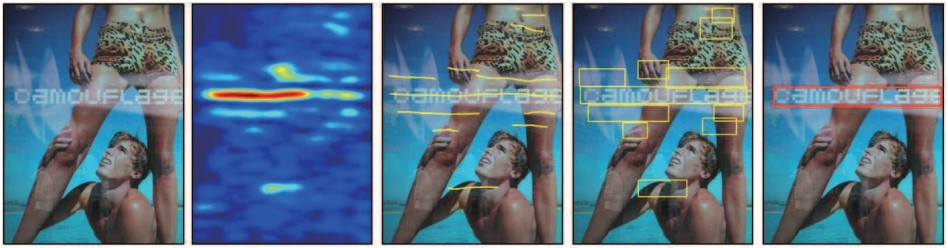
\includegraphics[width=\textwidth]{./figures/c2_zhang_cnn.jpg}
    \begin{minipage}[t]{0.18\linewidth}
    \centerline{ \small (a) 输入原图}
    \end{minipage}
    \begin{minipage}[t]{0.18\linewidth}
    \centerline{ \small (b) 概率图}
    \end{minipage}
    \begin{minipage}[t]{0.18\linewidth}
    \centerline{ \small (c) 对称轴}
    \end{minipage}
    \begin{minipage}[t]{0.18\linewidth}
    \centerline{ \small (d) 候选文本行}
    \end{minipage}
    \begin{minipage}[t]{0.18\linewidth}
    \centerline{ \small (d) CNN分类结果}
    \end{minipage}
    \caption{基于对称性文本行检测算法流程}
    \label{fig.c2_zhang_cnn}
    \end{figure*}

    Zhang等\cite{Zhang2015Symmetry} 提出一种利用滑动窗提取对称性特征的文字检测算法。该方法首先设计1 个对称性计算模板来计算滑动窗口内区域的梯度直方图、局部二值模式LBP 以及颜色等特征的相似度,然后将这些特征输入随机森林分类器从而得到每个像素属于文本行对称轴的概率图。接着把概率图上概率相近的像素集中形成文本行对称轴并用CRF 进行更准确的分类。然后在此基础上利用窗口尺寸生成候选文本行并作多个尺度上的文本行的投影融合。最后采用训练好的CNN分类器去掉非文字的图像区域。从这个方法的实验结果来看,利用深度学习来分类候选文本行区域,可将其中真实的文字部分精准的辨别出来,因而能较大程度的提高文本检测的成绩。

    \begin{table*}[!h]
    \centering
    \caption{基于区域的相关文字检测方法}
    \begin{tabular}{p{0.17\textwidth}|p{0.1\textwidth}| p{0.63\textwidth}}
    \hline
    作者 & 年份 & 方法概述 \\
    \hline
    Chen等\cite{Chen2004Detecting} & 2004 年 & 区域特征,滑动窗检测,以及SVM分类器;\\
    Pan等\cite{Pan2011A} & 2011年 &   条件随机场,滑动窗检测,以及waldBoost 分类器\\
    Wang等\cite{Wang2012End} & 2012 年 & 卷积神经网络和滑动窗检测 \\
    Zhang等\cite{Zhang2015Symmetry} & 2015 年 & 对称性特征,滑动窗检测以及卷积神经网络 \\
    \hline
    \end{tabular}
    \label{tab.c2_region_based}
    \end{table*}

    表格\ref{tab.c2_region_based}总结了基于区域的相关文字检测方法。基于区域方法的检测框架在图像上大多采用滑动窗进行细致的探索,并执行多尺度的处理来提取特征,因此甚至能在噪声环境中精准提取到文字。但相应地就会导致分类窗口过多的问题,故而计算量成倍增长,且对时间性能的要求也更苛刻。例如Wang等\cite{Wang2012End}提出的方法虽然取得极高的文字检测精度,但是其框架要求在原图的图像金字塔上进行多尺度的滑动窗扫描以提取候选文字图块区域,然后再将每个候选文字图块输入到CNN分类器中进行判别。这样一来即使是如$900\times1200$ 个像素大小的小规格图片,都要耗费几分钟的时间用来检测文字,因而根本无法投入实用。目前更流行的方法是诸如Zhang 等\cite{Zhang2015Symmetry} 的方法,也就是将传统模式识别方法与深度学习方法结合在一起,既充分挖掘了文字自身的特征,又获得了更精确的分类结果。而现在最值得研究的问题就是如何在确保文字检测精度的同时,还能进一步提高检测框架的效率。本文第\ref{sec.c3}章将会对该问题进行探讨。

    \section{基于连通部件的场景文字检测方法}
    \esection{Connected Component-based Method}

    基于连通部件的检测方法,将文字看做是一些连通部件的集合,所以这类方法是把连通部件作为处理对象的文字检测算法。这种基于连通部件来检测场景图像中文字的原理是:因为文字之间的笔画、纹理、对比度以及颜色等特征具有一致性,所以可通过笔画宽度转换、图像分割或最稳定极值区域提取等处理,来把候选文字的像素组成一系列的连通部件。

    \begin{figure}[!h]
    \centering
    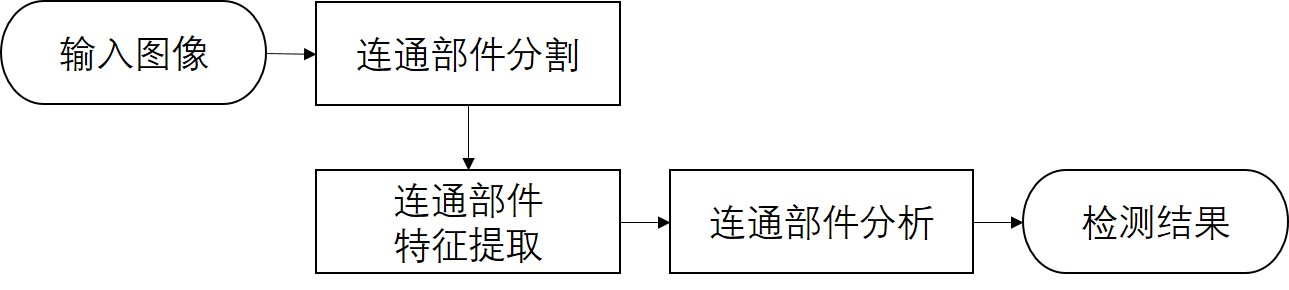
\includegraphics[width=\textwidth]{c2_cca_based.jpg}
    \caption{基于连通部件的文字检测方法的步骤示意图}
    \label{fig.c2_cca_based}
    \end{figure}

    如图\ref{fig.c2_cca_based}所示,这是一个典型的基于连通部件的检测方法的步骤示例。在此类方法的处理步骤中,通常首先会标记可能同属一个字符连通部件的像素,然后在分割连通部件的阶段通过把文字从背景中分离出来而得到候选的文字部件;接着在分析连通部件的阶段,首先提取笔画、几何、边缘及颜色等这些基于连通部件的特征,然后利用分类器来过滤掉非文字的部件;最后留下来的文字检测结果作为输出。

    Epshetein等\cite{Epshtein2010Detecting}提出用笔画宽度变换方法SWT来检测文字,促进了基于边缘(是连通部件中的一种)的文字检测算法的研究。这个方法根据图像里的文字笔画的宽度通常较为均一的属性,来过滤掉非文字边缘的像素。该方法首先利用Canny算子在场景文字图像的灰度图上求取图像中各目标的边缘,然后执行笔画宽度转换算法来计算笔画宽度图,其关键思路为:以边缘上的每个像素点为起始位置,沿该起始位置的梯度正负方向出发进行搜索,以找到梯度方向与起始位置点的方向近似相反的另一个边缘点,那么标记两像素点间的距离即为这个边缘的笔画宽度。在笔画宽度转换之后,再利用连通部件方法聚合起具有相近笔画宽度的像素点,以生成候选文字区域并方便后续的连通部件分析。最后使用启发性规则,例如欧拉数、宽高比等特征来过滤以得到真实文字区域。

    Yu等\cite{Yu2016Scene}是另一种基于边缘的文字检测方法。在该方法中,Yu 等人提出了一种基于边缘重组、边缘滤波和多通道处理的自然场景图像文本检测与定位方法。为了从背景中分割出文本,在边缘分析过程中首先将边缘分割为一个个单独的边缘段,然后将这些边缘段重新组合到候选字符的连通部件上,并利用边缘滤波器滤除大部分的背景边缘,那么剩余下来的候选字符边缘将被链接到候选文本行上即得到定位结果。文中使用两种不同的分类器来过滤掉非文本行,并且为了更准确地进行分类,作者首先将提取到的特征存储在特征池中,然后利用SVM 从特征池中选择最有效的特征来训练分类器。最后多通道用于确保文字检测查全率,而非极大抑制用来消除重复结果。

    \begin{figure*}[!h]
    \centering
    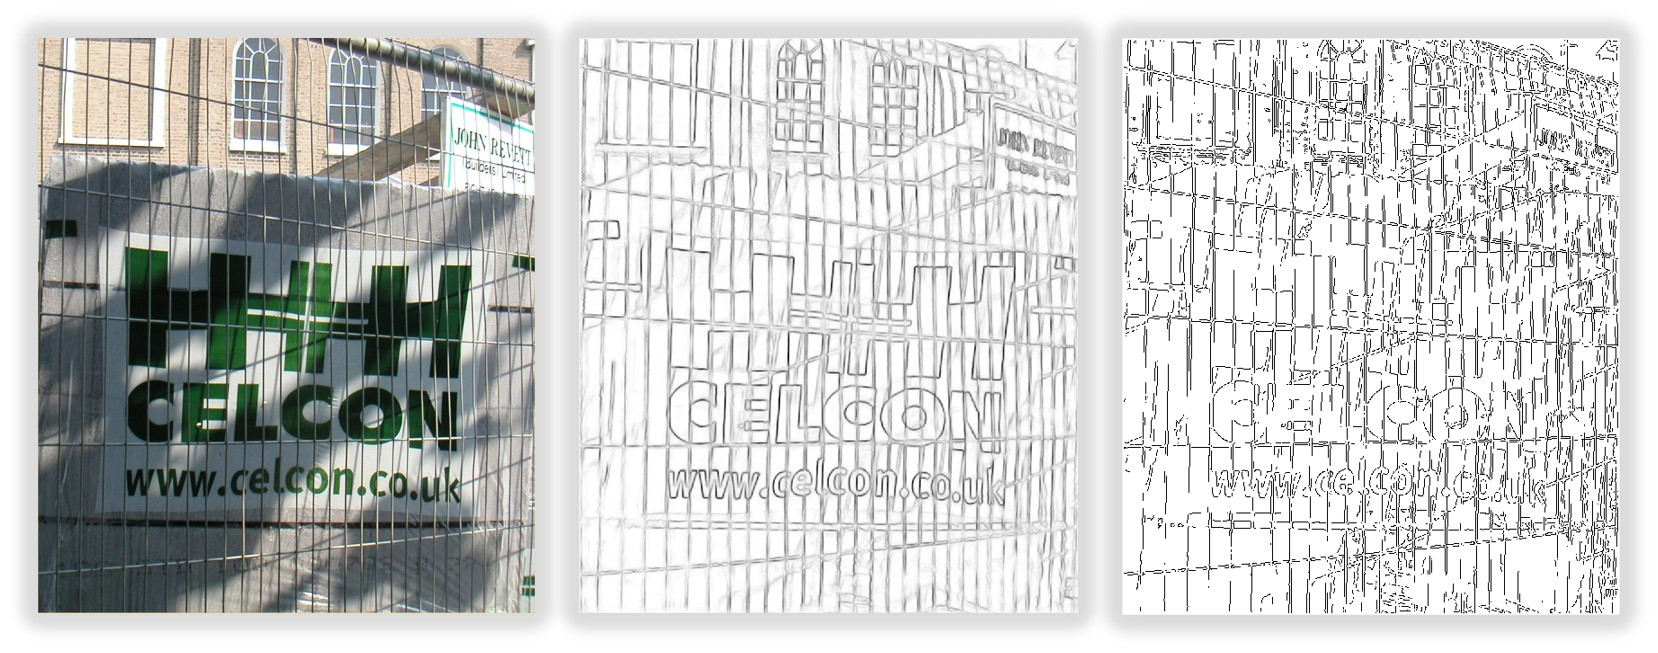
\includegraphics[width=\textwidth]{./figures/c2_sf_vs_canny.jpg}
    \begin{minipage}[t]{0.32\linewidth}
    \centerline{ \small (a) 原图}
    \end{minipage}
    \begin{minipage}[t]{0.32\linewidth}
    \centerline{ \small (b) 结构化边缘图}
    \end{minipage}
    \begin{minipage}[t]{0.32\linewidth}
    \centerline{ \small (a) Canny边缘}
    \end{minipage}
    \caption{基于结构化边缘检测算子和基于Canny 边缘检测算子的结果对比}
    \label{fig.c2_sf_vs_canny}
    \end{figure*}

    上述基于连通部件的方法中,对文字边缘的检测大多使用Canny 算子。而Dollar 等\cite{Dollar2015Fast} 提出一种新的结构化的边缘检测子。在这篇文章中,作者利用局部图像块中存在的结构来学习得到精确和高效的边缘检测器,并提出了一个应用于随机决策森林的结构化学习框架来预目标边缘掩码的问题。如图       \ref{fig.c2_sf_vs_canny}(b) 所示,用结构化边缘检测子求取的边缘图要比Canny 算子得到的如图\ref{fig.c2_sf_vs_canny}(c) 边缘图鲁棒且清晰得多。而进一步的,Zitnick 等\cite{Zitnick2014Edge} 提出的就是基于这种结构化边缘的目标检测方法,叫做edgebox边缘包围盒算法。作者认为边缘能够提供图像的稀疏但信息丰富的表示,因此这篇文章利用完全包含在包围盒中的边缘数目来指示该包围盒包含对象的概率。而这种目标检测方法也可以通过改进而应用到文字边缘的检测方法中,这部分内容会在第\ref{sec.c3_skeleton}节中作详细论述。

    \begin{figure*}[!h]
    \centering
    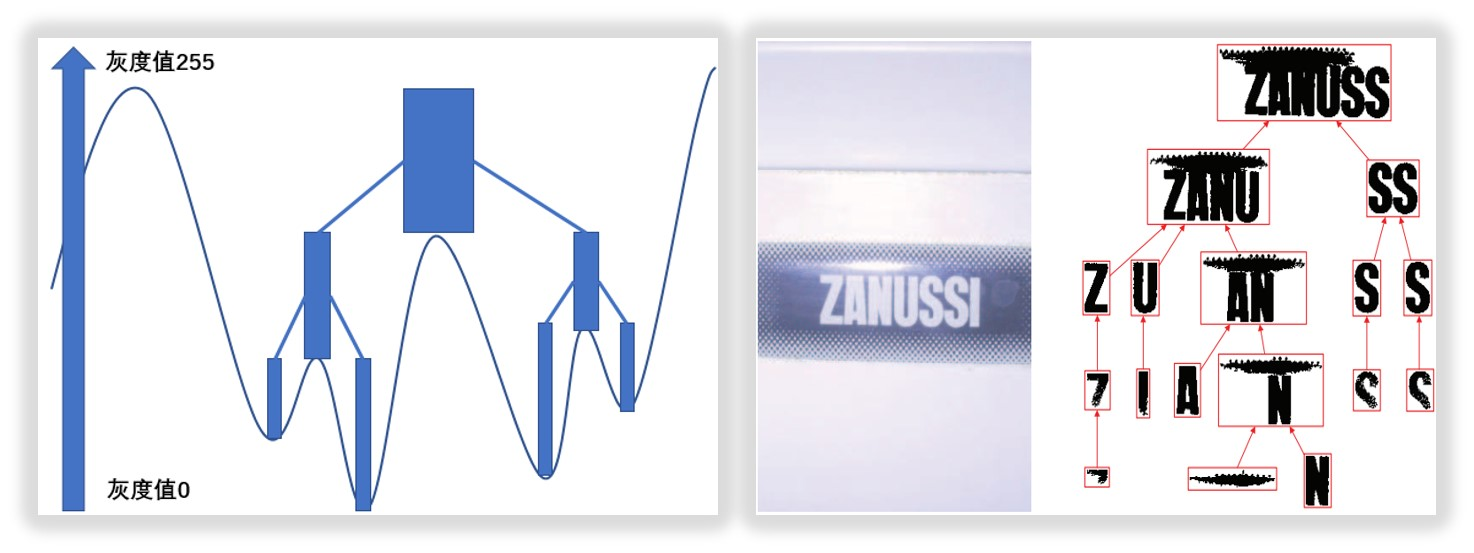
\includegraphics[width=\textwidth]{./figures/c2_er_tree.jpg}
    \begin{minipage}[t]{0.48\linewidth}
    \centerline{ \small (a) 分水岭算法}
    \end{minipage}
    \begin{minipage}[t]{0.48\linewidth}
    \centerline{ \small (b) 生成极值区域树}
    \end{minipage}
    \caption{生成极值区域树的示例图}
    \label{fig.c2_er_tree}
    \end{figure*}

    基于极值区域的方法是基于连通部件类方法中的另外一个比较经典和常见的文字检测方法。首先在文字检测方法中应用到最稳定极值区域MSER并获得显著的检测效果的是Neumann 等\cite{Neumann2010A} 提出的方法。而且Neumann 在其后续研究如\cite{Neumann2011Text}里坚持依据MSER 算法来提升文字检测算法的效果。MSER 算法的原理如下:首先极值区域ER 的概念即是区域外像素灰度值全部大于区域内部所有像素的区域,然后最稳定极值区域MSER 便是在极值区域ER 的基础上的图像分割方法。因为我们预设了候选文字目标的颜色均一并显著不同于背景,所以在对图像进行连续多个阈值的分割时,候选文字的目标区域面积会在一定阈值范围内呈现非常小的变化。

    接下来Neumann又在方法\cite{Neumann2012Real} 中反过来利用极值区域ER取代MSER以提取候选文字的连通部件,这是因为MSER 对于一些模糊或光照过强的场景太敏感而漏检掉了候选文字部件,但ER 却可以尽可能多的考虑到所有的连通部件,因为ER 本来涵盖了MSER 中所有的结果。生成ER 树的过程如图\ref{fig.c2_er_tree}(b)所示,其原理类似于图\ref{fig.c2_er_tree}(a)的分水岭算法。在这类算法中,主要是利用ER树提取候选的文字部件,然后求取连通部件的空洞面积、欧拉数、水平交叉数目以及紧密度等特征,来训练SVM 分类器以分类背景和文字。最后通过穷举搜索以将保留下来的连通部件排列成单词结果。

    \begin{table*}[!h]
    \centering
    \caption{基于连通部件的相关文字检测方法}
    \begin{tabular}{p{0.17\textwidth}|p{0.1\textwidth}| p{0.63\textwidth}}
    \hline
    作者 & 年份 & 方法概述 \\
    \hline
    Epshetein等\cite{Epshtein2010Detecting} & 2010 年 & 候选文字筛选,笔画宽度转换SWT,文本行生成;\\
    Neumann等\cite{Neumann2011Text} & 2011 年 &   最稳定极值区域MSER,穷举搜索\\
    Dollar等\cite{Dollar2015Fast} & 2015 年 & 结构化边缘检测子,随机森林分类器 \\
    Yu等\cite{Yu2016Scene} & 2016年 & 文字的特征池,文字的边缘重组,以及SVM 分类器 \\
    \hline
    \end{tabular}
    \label{tab.c2_connected_component_based}
    \end{table*}

    表格\ref{tab.c2_connected_component_based} 总结了基于连通部件的相关文字检测方法。基于连通部件的方法来提取候选文字的计算量要远远低于基于滑动窗的方法,因此这类方法的处理时间大为缩短,并且其检测到的结果可直接应用到识别文字的阶段。但基于连通部件的方法在曝光或低对比度环境中难以从背景中分离出连通区域,并且过于依赖图像分割算法的结果。Neumann 等\cite{Neumann2010A,Neumann2011Text,Neumann2012Real} 提出的MSER是其中的一大主流方法,该方法取得了不错的文字检测效果。但MSER也存在一些问题,如遭遇反光问题会失效、提取ER 时的重复和嵌套问题、以及过滤ER 时的固定阈值问题。因此目前在利用MSER 时大多先用一些其它方法作预处理以提高文字检测算法的鲁棒性。另一类主流的方法是如Yu 等\cite{Yu2016Scene}提出的基于边缘的文字检测框架。这类方法比较依赖边缘检测的效果,因此我们还用Yu 等\cite{Yu2016Scene} 提出的结构化边缘检测子取代了常用的Canny边缘检测算法。通过分析发现基于边缘的文字检测的最核心的问题是:若存在背景与文字边缘粘连问题,或不能完整提取文字边缘时,就很难进行后续的文字检测的分析,并造成漏检问题。针对这一问题,本文后续内容会作进一步的分析和改进。

    \section{本章小结}
    \esection{Brief Summary}

    本章分两部分来介绍和总结文字检测方法的相关理论和技术。首先介绍了基于区域的文字检测的经典方法,并总结了这类方法的优缺点和待解决的问题;然后介绍了另一类主流方法,即基于连通部件的文字检测方法,从中也分析了现有方法的不足,并作为本文提出方法的解决目标。

